\section{Synthetic Likelihoods}
\label{sec:sl}
There are two key motivators for exploring the use of Synthetic Likelihoods in this set-up. The first is that Model $\mathcal{A}$ has no (unconditioned) tractable likelihood function and the second is the double penalty effect. The first is caused by the regime-switching nature of the model. Following \cite{huisman_mahieu_2003}, separate likelihood functions could be obtained by conditioning on each regime. Then, the Kalman Filter could be applied to obtain Maximum Likelihood Estimates. However, there are good reasons to seek a method which does not require the Kalman Filter.

One reason is that the Kalman Filter puts restrictions on how the individual regimes can be specified. In particular, the Kalman Filter requires the model to be written in the form
\begin{equation}
    \begin{cases}
        \pmb{x}(t + 1) = \pmb{\Phi}(t + 1 ;t)\pmb{x}(t) + \pmb{u}(t) \\
        \pmb{y}(t) = \pmb{M}(t)\pmb{x}(t)
    \end{cases}
\end{equation}
where $\pmb{x}(t)$ is the state of the system, $\pmb{\Phi}(t + 1 ;t)$ is a transition matrix, $\pmb{u}(t)$ is a zero-mean Normal random variable, $\pmb{M}(t)$ is a matrix and $\pmb{y}(t)$ is the output of the system; all at time $t$ \citep{kalman_1960}. For Model $\mathcal{A}$, it means the distribution of the spikes must be Normal (Equation~\ref{eqn:spike}). This is an issue since the spikes should always be positive which under a Normal distribution will not always be the case. It is more appropriate to replace the Normal distribution with the Log-Normal distribution. This is possible with Synthetic Likelihoods but not with the Kalman Filter. In short, Synthetic Likelihoods offer the opportunity to expand upon Model $\mathcal{A}$ in useful and meaningful ways.

The second motivator for using Synthetic Likelihoods is the double penalty effect or `double penalty problem'. The classical `double penalty problem' refers to the modelling of rainfall. Specifically, a model that accurately predicts intensity, size and timing but is off on location incurs a `double penalty' with respect to point-wise error measures \citep{keil_craig_2009}.

In Model $\mathcal{A}$, the double penalty effect occurs in the following sense. First, the regime that the model is in on day $t$ is a hidden state. Thus, it is not known when the price spikes occur. Consider Figure~\ref{fig:double_penalty}. There are two trajectories. The observed trajectory and a simulated trajectory. The simulated trajectory has spikes of a similar magnitude and frequency to the spikes of the observed trajectory. This suggests the parameters used to generate the simulated trajectory are `good' parameters. Repeatedly sampling with these parameters would often produce similar situations to Figure~\ref{fig:double_penalty}. The simulations would have approximately the right number and size of spikes, but they would rarely coincide. This results in the double penalty effect.

\begin{figure}[H]
    \centering
    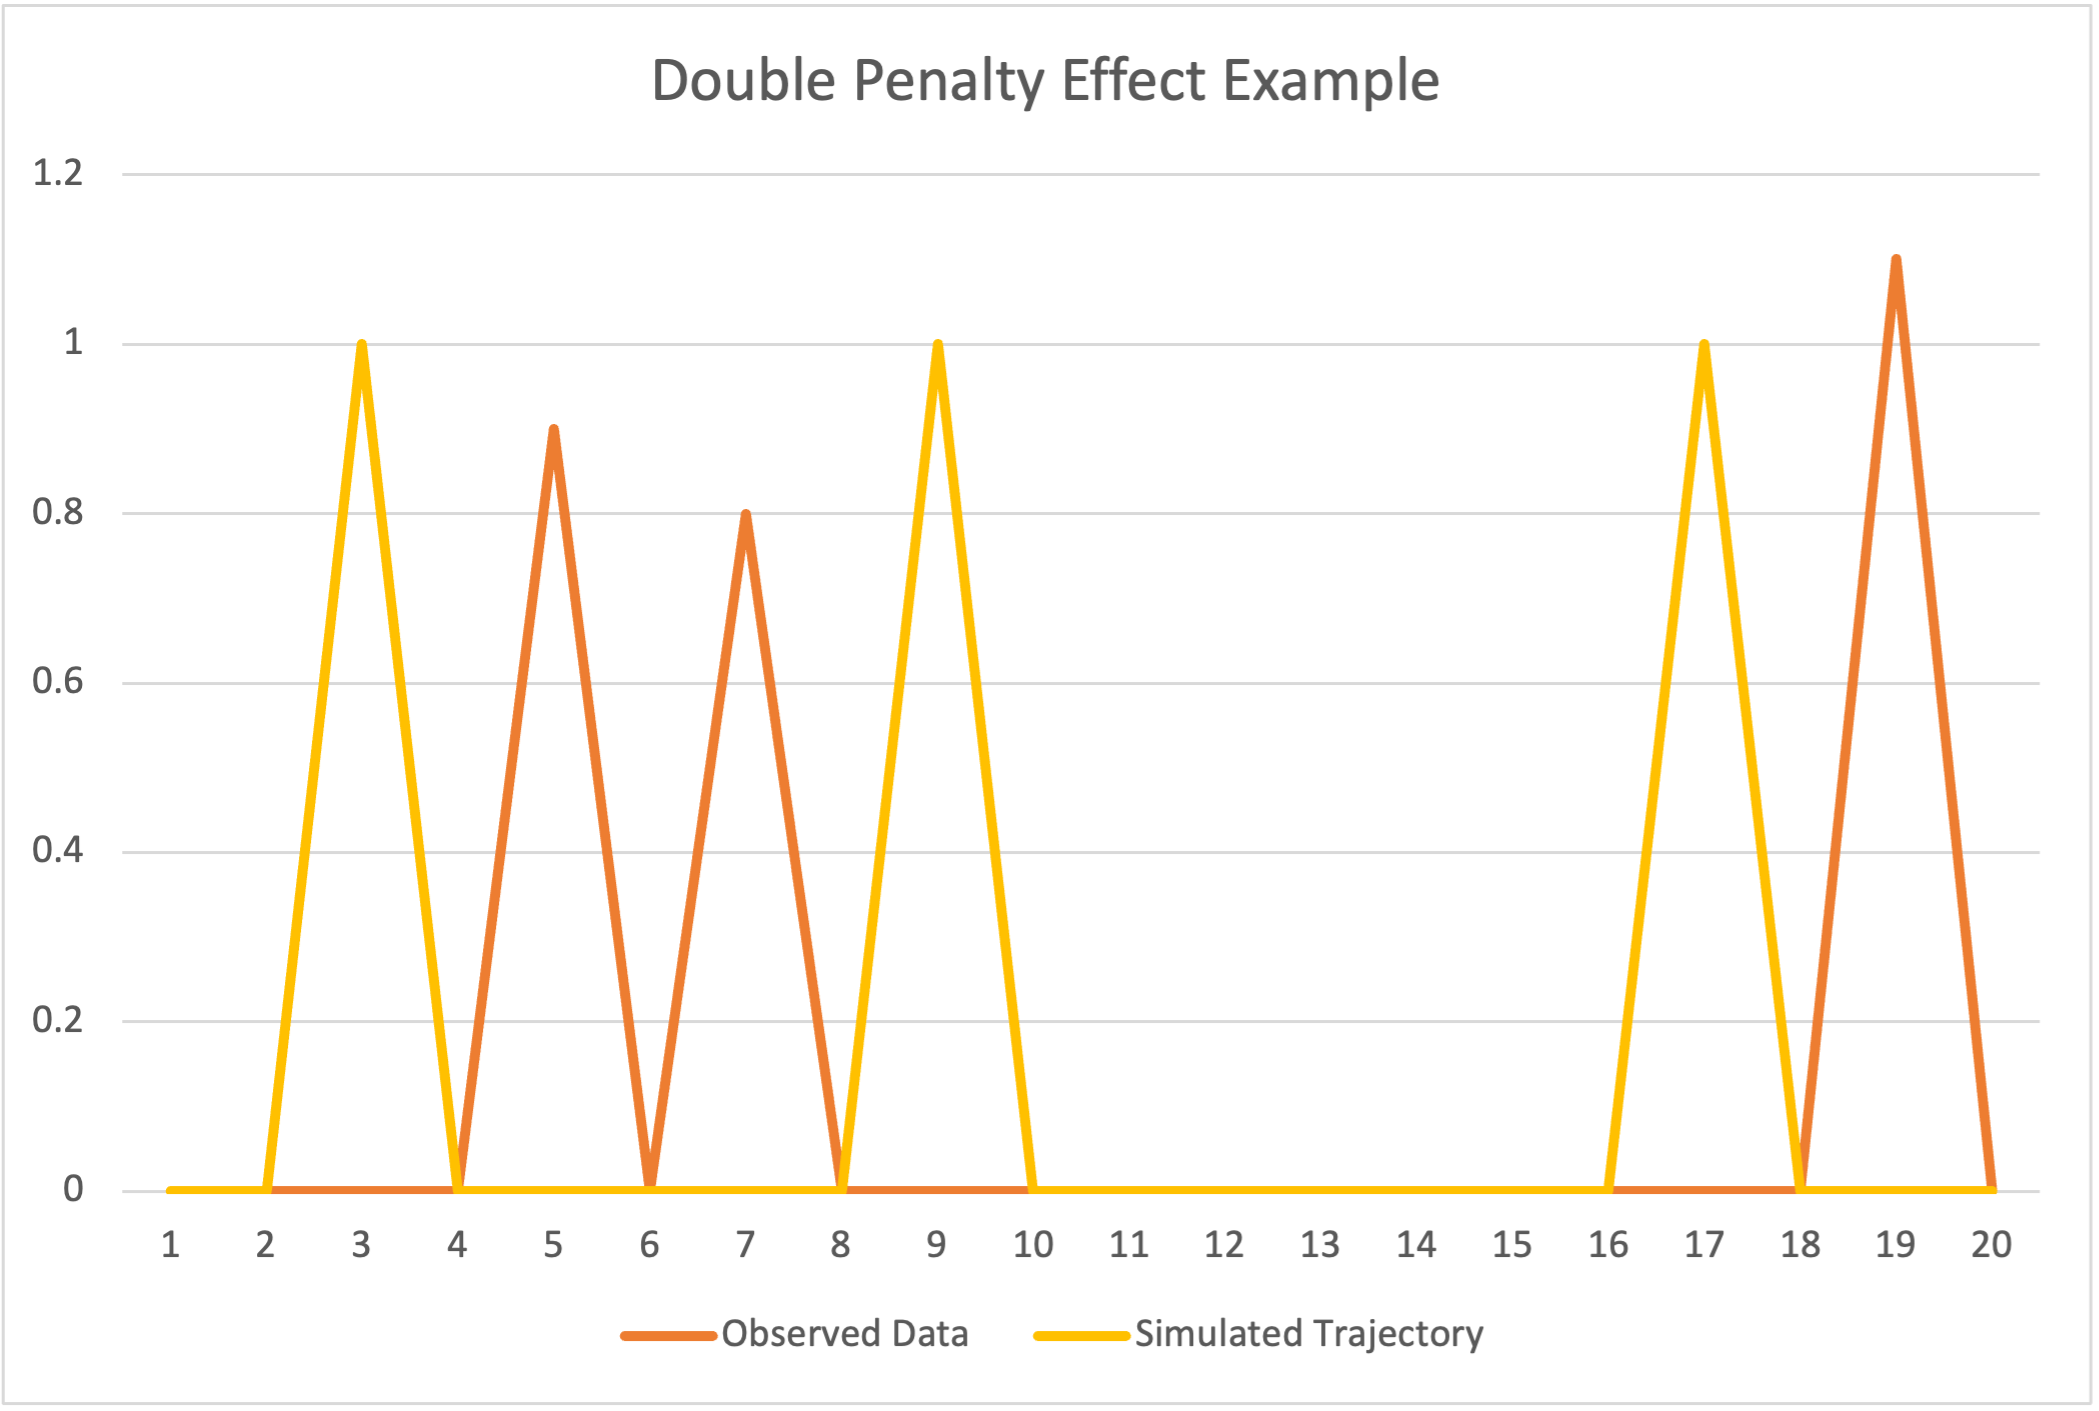
\includegraphics[width=12cm]{images/sl/double_penalty_excel.png}
    \caption{Double Penalty Effect \citep{haben_2014}}
    \label{fig:double_penalty}
\end{figure}

One solution would be to integrate out the hidden state from the joint density of the observations and the hidden state, as with the Kalman Filter. However, this is undesirable as it restricts how Model $\mathcal{A}$ can be specified. There may be particle filter algorithms that could accomplish this without restricting the specification of model $\mathcal{A}$, but they are computationally intensive and beyond the scope of this project. Thus, a method of parameter inference that does not require integrating out the hidden state is required.

Synthetic Likelihoods, as will be seen in Section~\ref{subsec:sl-method}, do not need a tractable likelihood function. Further the `double penalty' effect can be solved by only choosing statistics that are agnostic to the locations of the price spikes. There is no need to integrate out the hidden state. Now that there is sufficient motivation, Synthetic Likelihoods can be introduced.

\subsection{Synthetic Likelihood Estimation}
\label{subsec:sl-method}

Synthetic Likelihood Estimation will be introduced in comparison to Maximum Likelihood Estimation. With Maximum Likelihood Estimation, parameters are chosen to maximise the chance of producing the observed trajectory \citep[p.~226]{rossi_2018}. With Synthetic Likelihood Estimation, first summary statistics that characterise the dynamics of the model are selected, then parameters are chosen that maximise the likelihood of producing the observed summary statistics. To compute the likelihood, it is assumed that the summary statistics follow a multivariate Normal distribution.

Crucially, there is no need for a tractable likelihood function and the double penalty effect need not apply. The two requirements are a) the ability to sample from the model and b) to choose appropriate summary statistics.

The method is precisely defined in Algorithm~\ref{alg:sl} \citep{fasiolo_pya_wood_2016}.

\begin{singlespace}
\begin{algorithm}[H]
    \caption{Calculation of the Synthetic Likelihood}
    \label{alg:sl}
    \begin{algorithmic}
        \State Let $p(\pmb{y} | \pmb{\theta})$ be a statistical model
    
        \State Let $\pmb{y}^0$ be the observed trajectory
    
        \State Let $S(\cdot)$ be a function that computes the summary statistics of a trajectory
    
        \State Let $\pmb{s}^0 = S(\pmb{y}^0)$
    
        \State Assume $S(\pmb{y}) \sim \mathcal{N}(\pmb{\mu_\theta}, \pmb{\Sigma_\theta})$
        
        \State Let $\phi(\cdot)$ be the log-likelihood function of a multivariate Normal distribution
        \newline
        \Procedure{Synthetic\_Likelihood}{$p, S, N, \pmb{s}^0$}
            \State Simulate $N$ data sets $\pmb{y}^1, \ldots, \pmb{y}^N$ from the model $p(\pmb{y} | \pmb{\theta})$
            \State Calculate $\pmb{s}^i = S(\pmb{y}^i)$ for $1 \leq i \leq N$
            \State Calculate the sample mean $\hat{\pmb{\mu}}_{\pmb{\theta}}$ and sample covariance $\hat{\pmb{\Sigma}}_{\pmb{\theta}}$ of $\pmb{s}^1, \ldots, \pmb{s}^N$
            \State Estimate the Synthetic Likelihood $\hat{p}(\pmb{s}^0 | \pmb{\theta}) = \phi(\pmb{s}^0 | \hat{\pmb{\mu}}_{\pmb{\theta}}, \hat{\pmb{\Sigma}}_{\pmb{\theta}})$
            \State \Return $\hat{p}(\pmb{s}^0 | \pmb{\theta})$
        \EndProcedure
    \end{algorithmic}
\end{algorithm}
\end{singlespace}

To explore Synthetic Likelihood Estimation in more detail it will be used to infer the parameters of a Zero-Inflated Gamma distribution.

\subsection{Example: Zero-Inflated Gamma}
\label{subsec:gamma}

First, the Zero-Inflated Gamma random variable needs defining.

\begin{definition}
    Let $G \sim \text{Gamma}(\alpha, \beta)$, a Gamma random variable with shape parameter $\alpha$ and rate parameter $\beta$. Let $B \sim \text{Bernoulli}(p)$ where
    \[ p = \mathbb{P}(B = 1) = 1 - \mathbb{P}(B = 0). \]
    Then, X = (1-B)G, is a Zero-Inflated Gamma random variable with shape parameter $\alpha$, rate parameter $\beta$ and zero parameter $p$. In this case, write $X \sim \text{ZIG}(\alpha, \beta, p)$.
\end{definition}

With this definition, Synthetic Likelihood Estimation can be performed.

Let $X \sim \text{ZIG}(\alpha, \beta, p)$. For this example, choose the true parameters to be $\alpha^* = 3$, $\beta^* = 1$ and $p^* = 0.3$. Next, generate a sample of $m = 2000$ observations. This will be the observed trajectory denoted $\pmb{y}^0$. To construct the Synthetic Likelihood, summary statistics need to be chosen. Good choices of statistics include the sample mean and standard deviation since, for a Gamma distribution, these can be calculated in terms of $\alpha$ and $\beta$. Another useful statistic is the proportion of zeros which is needed to correctly infer the true value of $p$. Let $\bar{x}(\pmb{y}^i)$ denote the sample mean and $\text{sd}(\pmb{y}^i)$ the standard deviation of trajectory $\pmb{y}^i$. So for trajectory $\pmb{y}^i$, compute
\begin{equation}
S(\pmb{y}^i) = (\bar{x}(\pmb{y}^i), \text{sd}(\pmb{y}^i), \frac{1}{m}\sum_{j=1}^m \mathbb{I}\{y^i_j = 0\}).
\end{equation}
To estimate the Synthetic Likelihood for a given $\pmb{\theta} = (\alpha, \beta, p)$, do the following. Take $N=100$ samples and transform each sample to a summary statistic by $S(\cdot)$. Then, calculate the sample mean $\hat{\pmb{\mu}}_{\pmb{\theta}}$ and the sample covariance $\hat{\pmb{\Sigma}}_{\pmb{\theta}}$ of the summary statistics. Finally, compute $\hat{p}(\pmb{s}^0 | \pmb{\theta}) = \phi(\pmb{s}^0 | \hat{\pmb{\mu}}_{\pmb{\theta}}, \hat{\pmb{\Sigma}}_{\pmb{\theta}})$ where $\pmb{s}^0 = S(\pmb{y}^0)$.

An estimate of the Synthetic Likelihood can now be computed for any $\pmb{\theta}$. To compute Synthetic Likelihood Estimate $\hat{\pmb{\theta}}$, a stochastic optimiser is needed to maximise the Synthetic Likelihood over all $\pmb{\theta}$. The `ML' optimiser from \emph{Synlik} \citep{synlik_2014} will do this. Implementing the above in R will result in convergence to the true parameters. This is shown in Figure~\ref{fig:no_robust_zig}.

\begin{figure}[H]
    \centering
    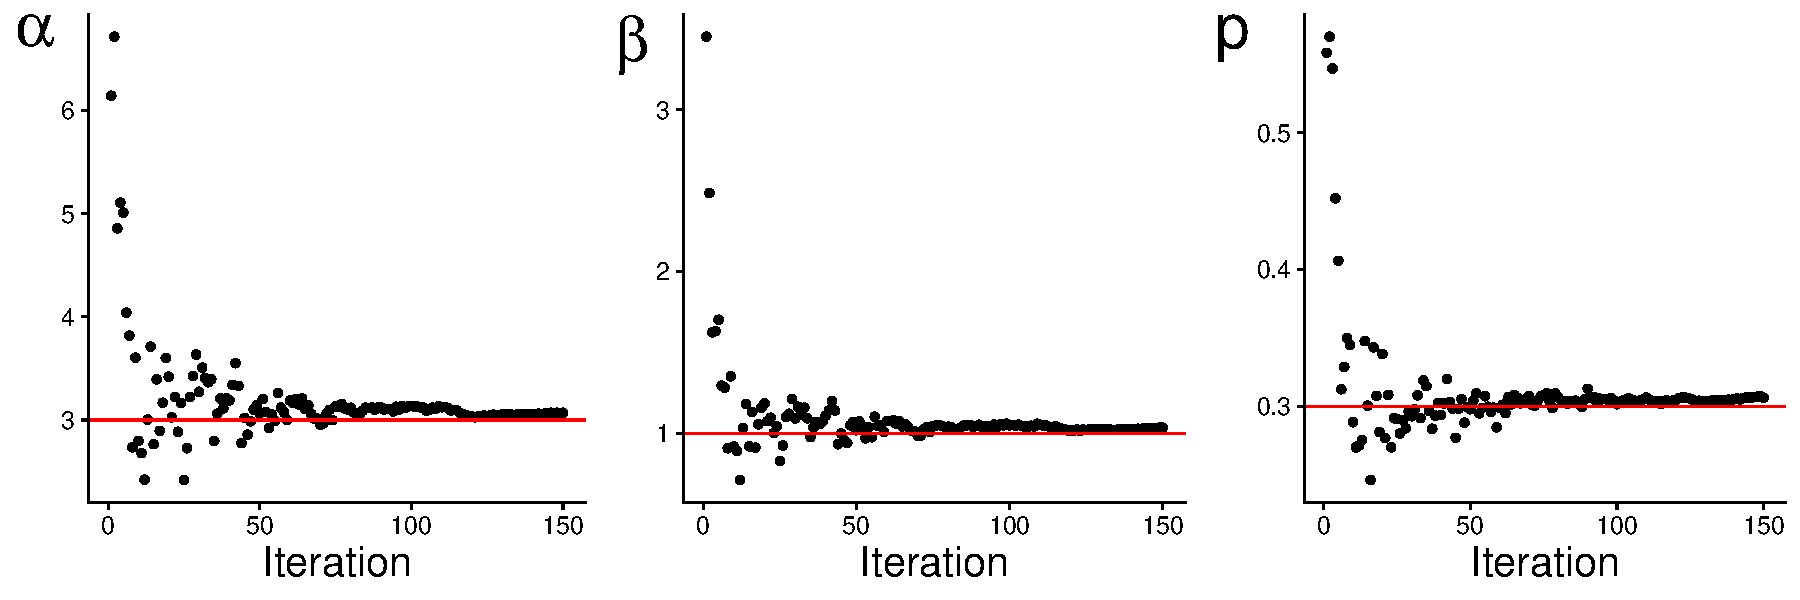
\includegraphics[width=12cm]{images/sl/gamma_example/no_robust_optimisation.pdf}
    \caption{Convergence to True Parameters (ZIG no RCM)}
    \label{fig:no_robust_zig}
\end{figure}

Synthetic Likelihood Estimation is a computationally intensive operation. This is due to the large number of samples that need to be generated to evaluate the likelihood at each stage of the optimisation. In this example, $50$ Synthetic Likelihoods were simulated at each stage of the optimisation and each Synthetic Likelihood generated $100$ samples. Thus, the entire optimisation generated $150 \times 50 \times 100 = 750000$ samples. This does not pose a problem for the ZIG example as the number of statistics is small. However, as the number of statistics grows, this becomes a significant issue as more samples are required to obtain a less noisy estimate of $\hat{\pmb{\Sigma}}_{\pmb{\theta}}$. In the next section, the Robust Covariance Matrix (RCM) will be introduced. This will reduce the number of samples required per likelihood to \emph{one}.

\subsection{Robust Covariance Matrix}
\label{subsec:rcm}
To motivate this section notice that, in Algorithm~\ref{alg:sl}, $\hat{\pmb{\mu}}_{\pmb{\theta}}$ could be estimated by simply evaluating the statistics over a sufficiently long trajectory. The Robust Covariance Matrix can be used in the same way to estimate $\hat{\pmb{\Sigma}}_{\pmb{\theta}}$. Thus, only one sample is needed to produce a likelihood. However, in order to use the Robust Covariance Matrix, only a certain class of statistics can be used - $M$-Estimators \citep{huber_1967}.

\begin{definition}
    An $M$-Estimator is a solution $\theta$ that minimises $L = \sum_{i=1}^n \rho(x_i, \theta)$ where $\rho$ is an arbitrary function.
\end{definition}

In Section~\ref{subsec:theoretical-properties}, it will be shown that $M$-Estimators are asymptotically Normal. As an example of an $M$-Estimator, it will be shown that any Maximum Likelihood Estimator is an $M$-Estimator.

\begin{proposition}
    \label{prop:mle-is-m}
    Any Maximum Likelihood Estimator is an $M$-Estimator.
\end{proposition}

\begin{proof}
Let $X_1, X_2, \ldots, X_n$ be a sequence of independent and identically distributed random variables with density $f(x|\theta)$ where $\theta$ is a parameter. Let $x_1, x_2, \ldots, x_n$ be the realisations of those  respective random variables. Then, the Maximum Likelihood Estimator for $\theta$ is given by
\[ \hat{\theta} = \argmax_{\theta\in \Theta} \left[ \text{log }  \prod_{i=1}^n f(x_i|\theta) \right] = \argmin_{\theta\in \Theta} \left[ \sum_{i=1}^n -\text{log } f(x_i|\theta) \right].\]
Thus, taking $\rho(x_i, \theta) = -\text{log } f(x_i | \theta)$ demonstrates that the Maximum Likelihood Estimator of $\theta$ is an $M$-Estimator.
\end{proof}

In order to define the Robust Covariance Matrix, the sample covariance is needed. The definition below is from \cite{krzanowski_2000}. 

\begin{definition}
    \label{def:cov}
    Let $\pmb{M} \in \mathbb{R}^{m \times n}$ be a matrix where $(\pmb{M})_{ij}$ is the $i$'th observation of the $j$'th variable. Obtain matrix $\pmb{Q}$ by subtracting the sample column means of $\pmb{M}$ from each column of $\pmb{M}$. Then, obtain the sample covariance as
    \[ \text{cov}(\pmb{M}) = \frac{1}{n-1} \pmb{Q}^T \pmb{Q}. \]
\end{definition}

In Definition~\ref{def:cov}, $\pmb{Q}^T$ represents the transpose of matrix $\pmb{Q}$.

Now the Robust Covariance Matrix can be defined. This project will modify the definition of the Robust Covariance Matrix given in \cite{huber_1967}.

\begin{definition}
    \label{def:rcm}
    Let $\pmb{y}^1$ be a sample trajectory with length $m$. Let $\pmb{s} \in \mathbb{R}^N$ be a vector of $N$ $M$-Estimators where $L_i$ is the corresponding loss-function for $M$-Estimator $s_i$ ($1 \leq i \leq N$). Let $L = \sum_{i=1}^N L_i$. Then, the Robust Covariance Matrix of $\pmb{s}$ is given by
    \[ \tilde{\pmb{\Sigma}}(\pmb{s}) = \pmb{H}_L^{-1}(\pmb{s}) \pmb{V}_{L}(\pmb{s}) \pmb{H}_{L}^{-1}(\pmb{s}) \]
    where $\pmb{H}_{L}$ is the Hessian matrix of $L$ and $\pmb{V}_{L}$ is the sample covariance of the gradient $\nabla L$ taken over $y_i^1$, $1 \leq i \leq m$. That is $\pmb{V}_{L}(\pmb{s}) = \text{cov}(\pmb{M}_{L}(\pmb{s}))$ where
    \[ \pmb{M}_{L}(\pmb{s}) = \begin{pmatrix}
    \text{---} & (\nabla L(\pmb{s}))|_{y^1_1} & \text{---} \\
    \text{---} & (\nabla L(\pmb{s}))|_{y^1_2} & \text{---} \\
    \vdots & \vdots & \vdots \\
    \text{---} & (\nabla L(\pmb{s}))|_{y^1_m} & \text{---} \end{pmatrix}. \]
\end{definition}

In Definition~\ref{def:rcm}, $(\nabla L(\pmb{s}))|_{y^1_i}$ refers to the gradient $\nabla L(\pmb{s})$ evaluated at the point of the trajectory $y^1_i$.

All the statistics chosen in the Zero-Inflated Gamma example are $M$-Estimators. Therefore, the Robust Covariance Matrix can be applied to the Zero-Inflated Gamma example.

\subsection{Example: Zero-Inflated Gamma Continued}
The setup is identical to before. Start with a $\text{ZIG}(\alpha, \beta, p)$ random variable where $\alpha^*=3$, $\beta^*=1$ and $p^*=0.3$, obtain the observed trajectory $\pmb{y}^0$ and calculate the vector of observed summary statistics $\pmb{s}^0 = S(\pmb{y}^0)$. Now, construct the likelihood function. First, a single sample, denoted $\pmb{y}^1$, is generated. Take
\begin{equation}
\hat{\pmb{\mu}}_{\pmb{\theta}} = \pmb{s}^1 = S(\pmb{y}^1)
\end{equation}
and
\begin{equation}
\hat{\pmb{\Sigma}}_{\pmb{\theta}} \approx \tilde{\pmb{\Sigma}}(\pmb{s}^1) = \pmb{H}_L^{-1}(\pmb{s}^1) \pmb{V}_{L}(\pmb{s}^1) \pmb{H}_{L}^{-1}(\pmb{s}^1)
\end{equation}
where $L$ is the loss function corresponding to $S(\cdot)$, the vector of summary statistics.
To find $L$, each statistic must be written as a solution to the minimisation of a loss function. Recall the statistics are
\begin{equation}
S(\pmb{y}^i) = (\bar{x}(\pmb{y}^i), \text{sd}(\pmb{y}^i), \frac{1}{m}\sum_{j=1}^m \mathbb{I}\{y^i_j = 0\}).
\end{equation}
Since sample mean $\bar{x}(\pmb{y}^i)$ and standard deviation $\text{sd}(\pmb{y}^i)$ are Maximum Likelihood Estimators, they are $M$-Estimators as per Proposition \ref{prop:mle-is-m}. In particular, they are the solution $(\xi_1, \xi_2) = (\bar{x}(\pmb{y}^i), \text{sd}(\pmb{y}^i))$ to the minimisation of
\begin{equation}
L_{1,2}(\xi_1, \xi_2) = -\sum_{i=1}^m \text{log}(f(y_i^1 \mid \xi_1, \xi_2^2))
\end{equation}
where $f$ is the density of a Normal distribution with mean $\xi_1$ and standard deviation $\xi_2$. For the proportion of zeros statistic, a quadratic loss function where $\xi_3 = \frac{1}{m}\sum_{j=1}^m \mathbb{I}(y^i_j = 0)$ is the solution to the minimisation of
\begin{equation}
L_3(\xi_3) = \frac{1}{2} \sum_{i=1}^m (\xi_3 - \mathbb{I}\{y^1_i = 0\})^2
\end{equation}
can be used. Therefore the loss function is
\begin{equation}
L(\xi_1, \xi_2, \xi_3) =  -\sum_{i=1}^m \text{log}(f(y_i^1 \mid \xi_1, \xi_2^2)) + \frac{1}{2} \sum_{i=1}^m (\xi_3 - \mathbb{I}\{y^1_i = 0\})^2.
\end{equation}
Now the Hessian and the covariance of the gradient of $L$, evaluated at $(\xi_1, \xi_2, \xi_3) = \pmb{s}^1$, are needed. By the chain rule, the gradient of $L$ for a single $y^1_i$ is
\begin{equation}
(\nabla L(\xi_1, \xi_2, \xi_3))|_{y^1_i} = (-\frac{y_i^1 - \xi_1}{\xi_2^2}, \frac{\xi_2^2 - (y_i^1 - \xi_1)^2}{\xi_2^3},\xi_3 - \mathbb{I}\{y^1_i = 0\}).
\end{equation}
Then, taking the covariance over all observations yields
\begin{equation}
\pmb{V}_L(\xi_1, \xi_2, \xi_3) = \text{cov} \begin{pmatrix}
    \text{---} & (\nabla L(\xi_1, \xi_2, \xi_3))|_{y^0_1} & \text{---} \\
    \text{---} & (\nabla L(\xi_1, \xi_2, \xi_3))|_{y^0_2} & \text{---} \\
    \vdots & \vdots & \vdots \\
    \text{---} & (\nabla L(\xi_1, \xi_2, \xi_3))|_{y^0_m} & \text{---}
\end{pmatrix}.
\end{equation}
The Hessian can be computed numerically. To compute the Synthetic Likelihood:
\begin{enumerate}
    \item Simulate the trajectory $\pmb{y}^1$
    \item Compute $\hat{\pmb{\mu}} = \pmb{s}^1 = S(\pmb{y}^1)$
    \item Plug in $\pmb{s}^1$ for $(\xi_1, \xi_2, \xi_3)$ to estimate $\hat{\pmb{\Sigma}}_{\pmb{\theta}} \approx \tilde{\pmb{\Sigma}}(\pmb{s}^1) = \pmb{H}_L^{-1}(\pmb{s}^1) \pmb{V}_{L}(\pmb{s}^1) \pmb{H}_{L}^{-1}(\pmb{s}^1)$
    \item Obtain the Synthetic Likelihood $\hat{p}(\pmb{s}^0 | \pmb{\theta}) = \phi(\pmb{s}^0 | \pmb{s}^1, \tilde{\pmb{\Sigma}}(\pmb{s}^1))$
\end{enumerate}
Again, this likelihood function can be passed to the `ML' optimizer from \emph{Synlik} \citep{synlik_2014} to produce the estimate $\hat{\pmb{\theta}}$. Convergence to the true parameters is still achieved and shown in Figure~\ref{fig:robust_zig}. Noteably, this happens much faster (time wise) since $100 \times$ fewer samples are used.

\begin{figure}[H]
    \centering
    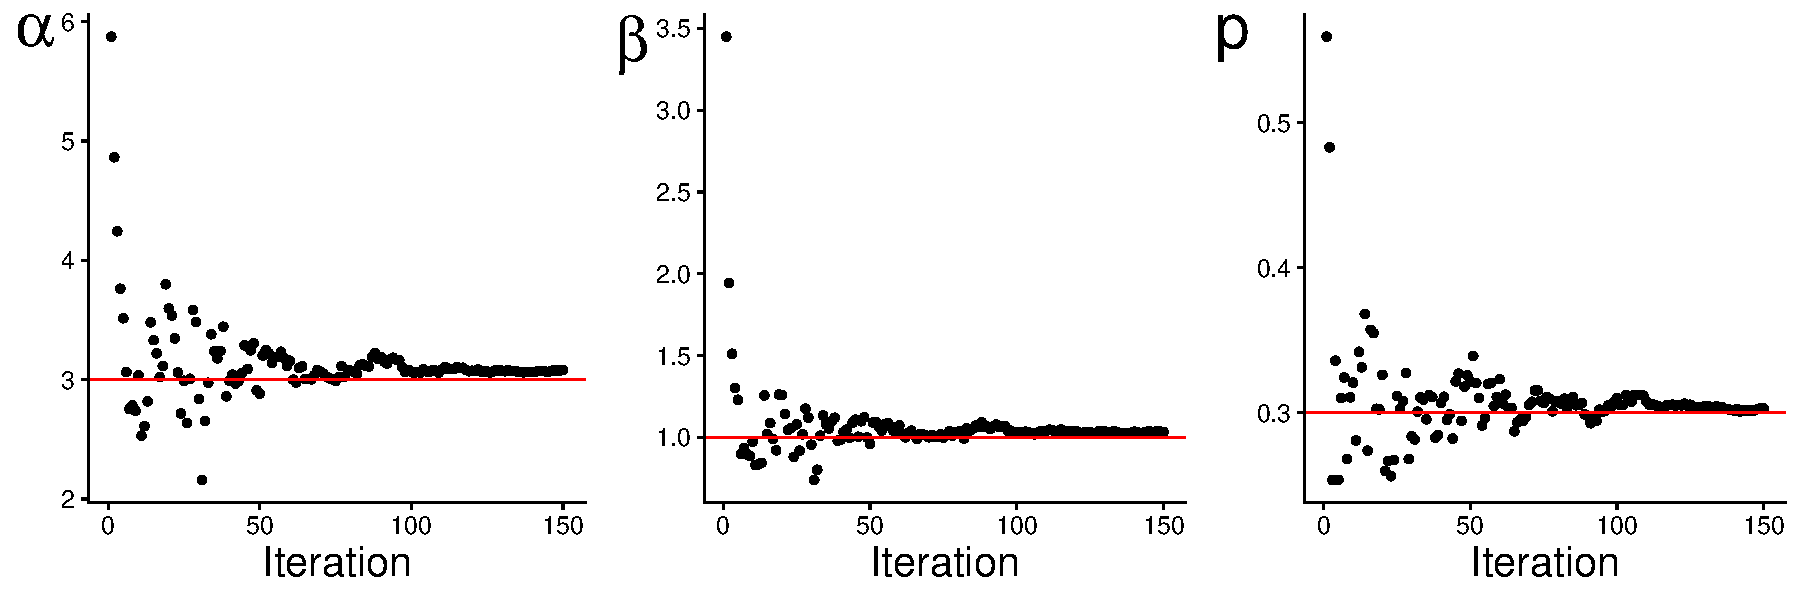
\includegraphics[width=12cm]{images/sl/gamma_example/robust_optimisation.pdf}
    \caption{Convergence to True Parameters (ZIG with RCM)}
    \label{fig:robust_zig}
\end{figure}

The next section will propose a heuristic for determining whether a set of statistics are likely to provide a good Synthetic Likelihood Estimate of the parameters.

\subsection{What is a Good Statistic?}
\label{subsec:corr_diag}

A good statistic must have the following two characteristics:

\begin{enumerate}
    \item high correlation with model parameters; and
    \item low correlation with other statistics.
\end{enumerate}

The first criterion ensures the statistics provide meaningful information about the model parameters. The second criterion is desirable as too much mutual correlation could result in singular covariance matrices. Thus, correlation diagrams, as shown in Figure~\ref{fig:corr_diags}, can be produced to build an idea for how a set of statistics may perform. These are particularly useful since it is far more computationally efficient to compute correlations than it is to perform Synthetic Likelihood Estimation.

\begin{figure}[H]
    \centering
    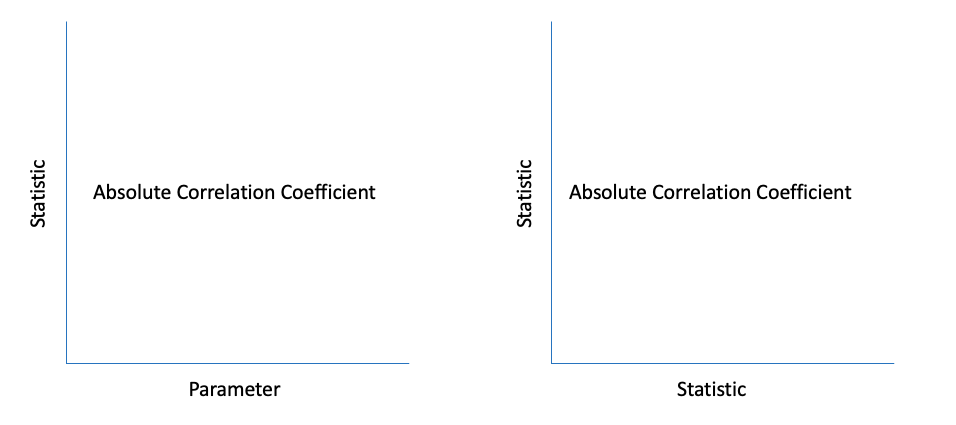
\includegraphics[width=10cm]{images/sl/corr_diags.png}
    \caption{Correlation Diagrams}
    \label{fig:corr_diags}
\end{figure}

Concretely, to produce these diagrams, choose sample parameters $\pmb{\theta}$ and covariance matrix $\Sigma$. Then, several sets of parameters from $\mathcal{N}(\pmb{\theta}, \Sigma)$, a multivariate Normal distribution, are sampled. For each set of parameters, an observed trajectory is produced and its summary statistics evaluated. The correlations between mutual statistics and between statistics and parameters can then be computed. Algorithm~\ref{alg:cor_diag} defines this process precisely. For notation, the $i$'th row of matrix $X$ is denoted by $X_{i*}$ and the $j$'th column by $X_{*j}$.

\begin{singlespace}
    \begin{algorithm}[H]
        \caption{Correlation Diagrams}
        \label{alg:cor_diag}
        \begin{algorithmic}
            \State Let $\pmb{\theta}$ and $\Sigma$ be the parameters of the multivariate Normal distribution from which model parameters will be drawn
            \State Let $f(\cdot)$ be a function that computes a random trajectory for some given parameters
            \State Let $S(\cdot)$ be a function that computes the statistics for a given trajectory
            \State Let $n$ be the number of parameters to sample and $m$ be the number of statistics computed by $S(\cdot)$
            \newline
            \Procedure{stat\_cor}{$\pmb{\theta}, \Sigma, f, S, n, m$}
                \State $P \gets n$ samples from $\mathcal{N}(\pmb{\theta}, \Sigma)$
                \State $S \gets $ Empty matrix of dimensions $n \times m$
                \For{$i \gets 1:n$}
                    \State $\pmb{t} \gets f(P_{i*})$
                    \State $S_{i*} \gets S(\pmb{t})$
                \EndFor
                \State $C \gets $ Empty matrix of dimensions $m \times \text{dim}(\pmb{\theta})$
                \For{$i \gets 1:\text{dim}(\pmb{\theta})$}
                    \For{$j \gets 1:m$}
                        \State $C_{ji} = |\text{cor}(P_{*i}, S_{*j})|$
                    \EndFor
                \EndFor
                \State $D \gets |\text{cor}(S)|$
                \State \Return $C, D$
            \EndProcedure
            \newline
            \State Note: $C$ is the matrix of correlations between statistics and parameters whereas $D$ is the matrix of correlations between statistics mutually.
        \end{algorithmic}
    \end{algorithm}
\end{singlespace}

Speaking from experience, it is best to first obtain a set of statistics that have strong correlations with all model parameters. Then, if Synthetic Likelihood Estimation fails, remove the most correlated statistics and repeat.

These diagrams can be computed for the Zero-Inflated Gamma Example. They are displayed in Figure~\ref{fig:zigcd}. Each parameter is correlated with at least one of the statistics. There is correlation between the mean and standard deviation statistics but this is not enough to upset the Synthetic Likelihood Estimation.

\begin{figure}[H]
        \centering
        \subfloat{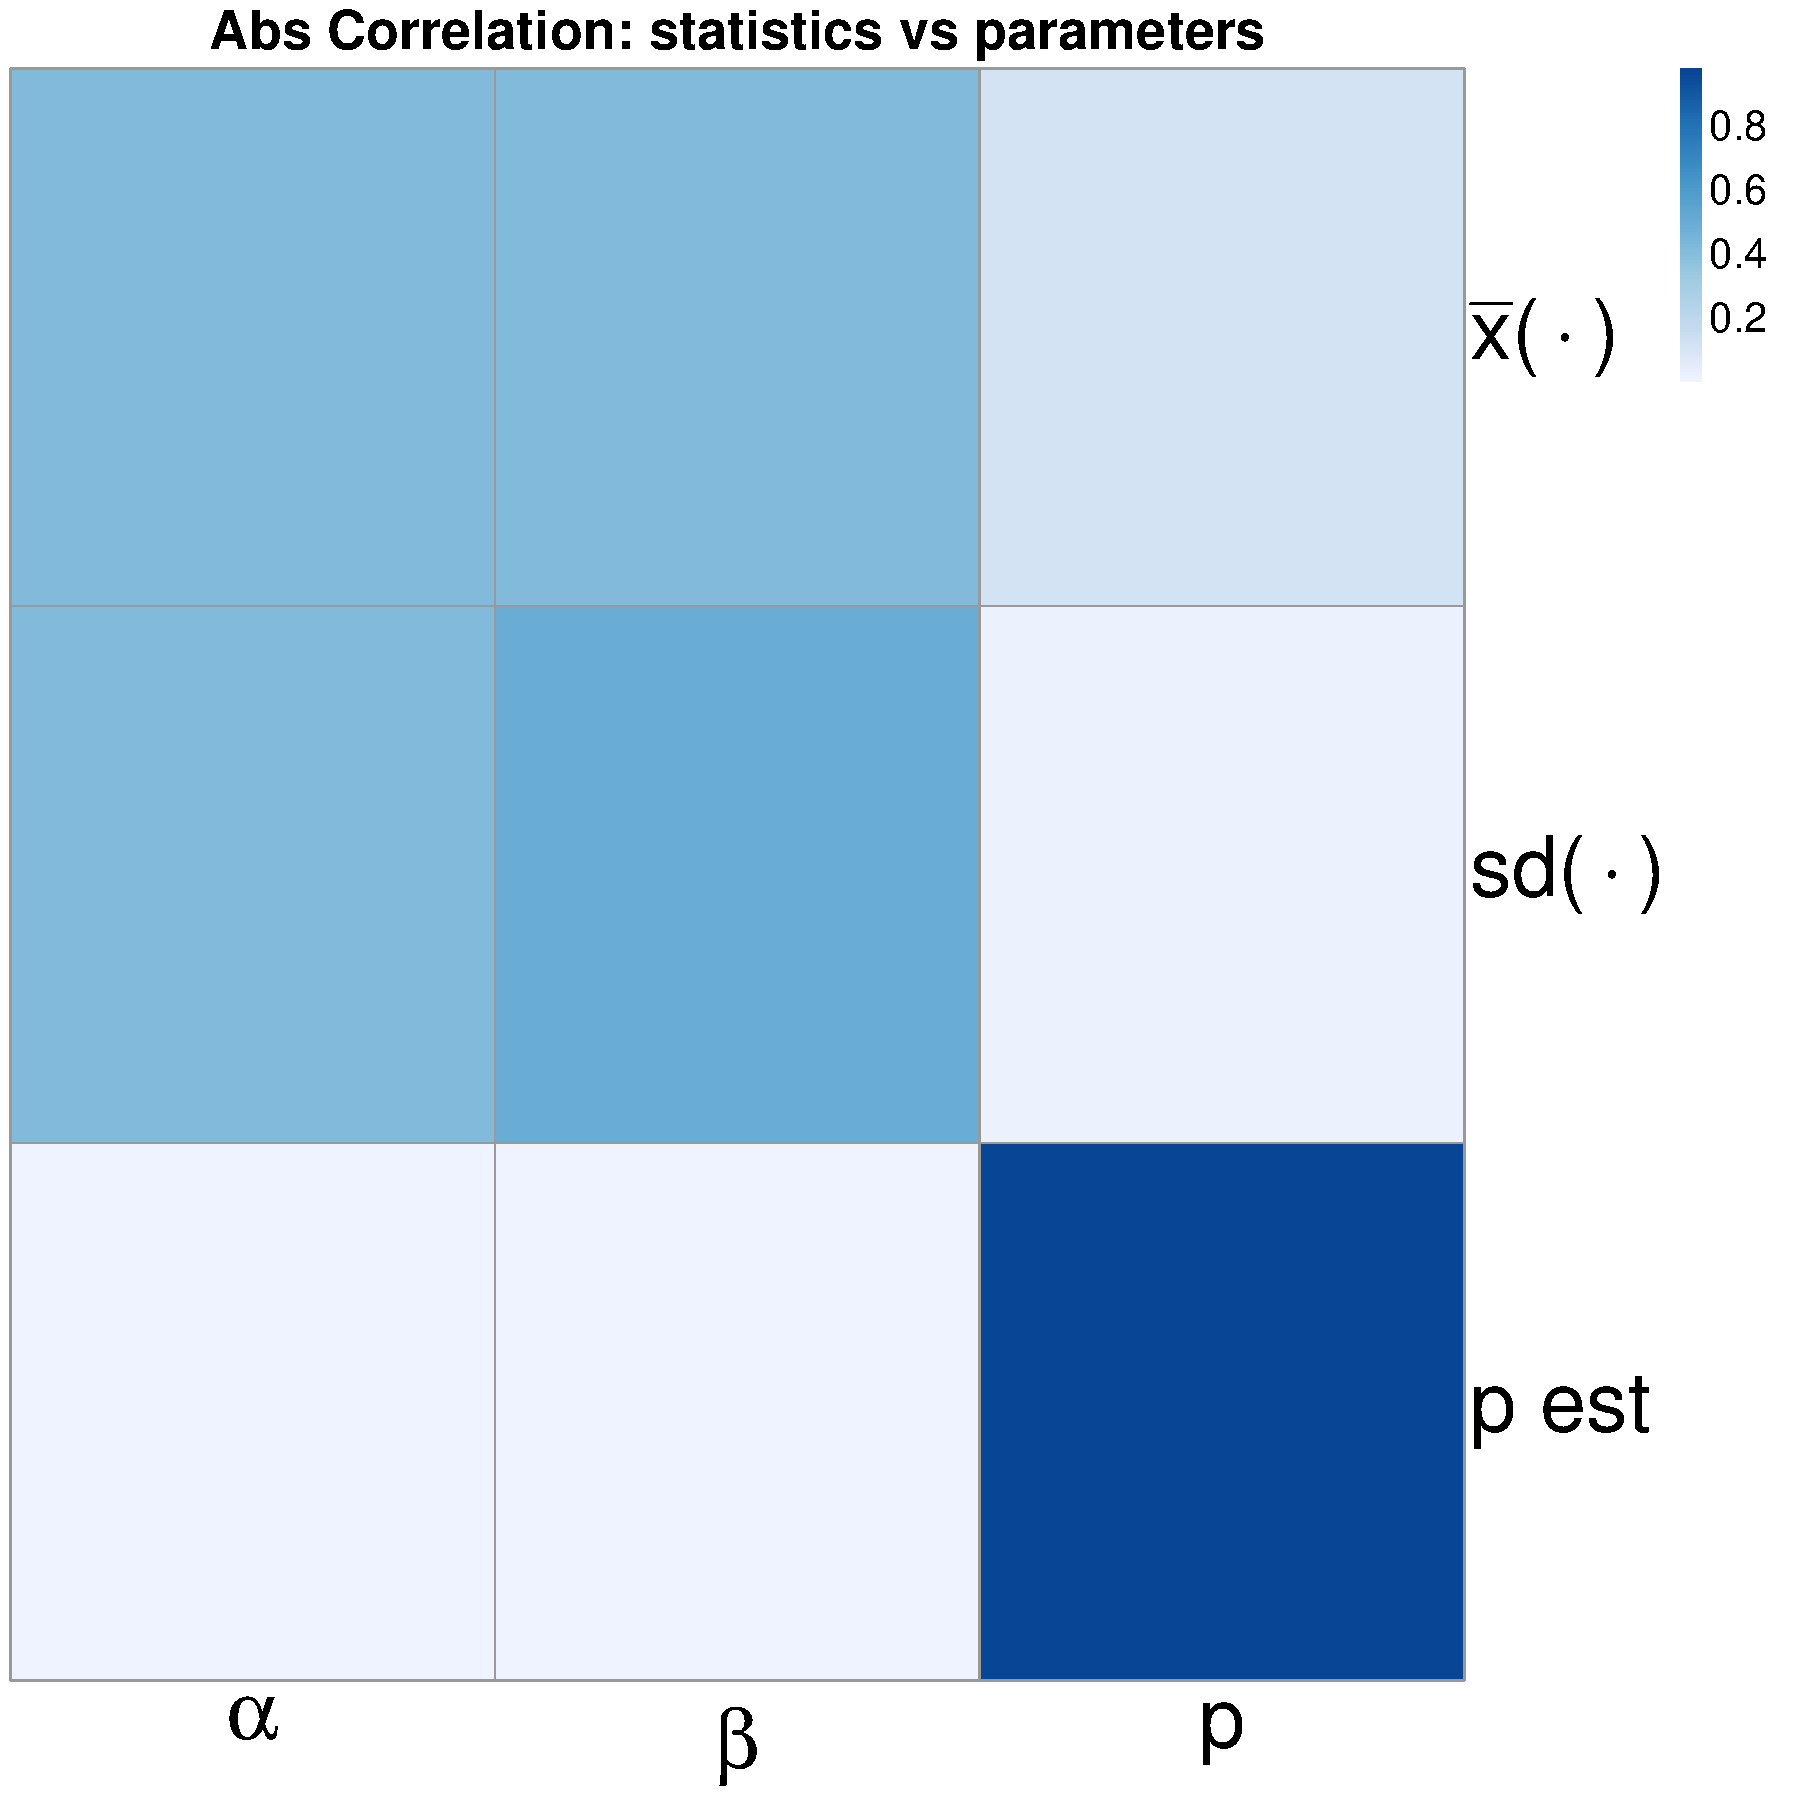
\includegraphics[width=55mm]{images/sl/gamma_example/cor_sp.pdf}}
        \qquad
        \subfloat{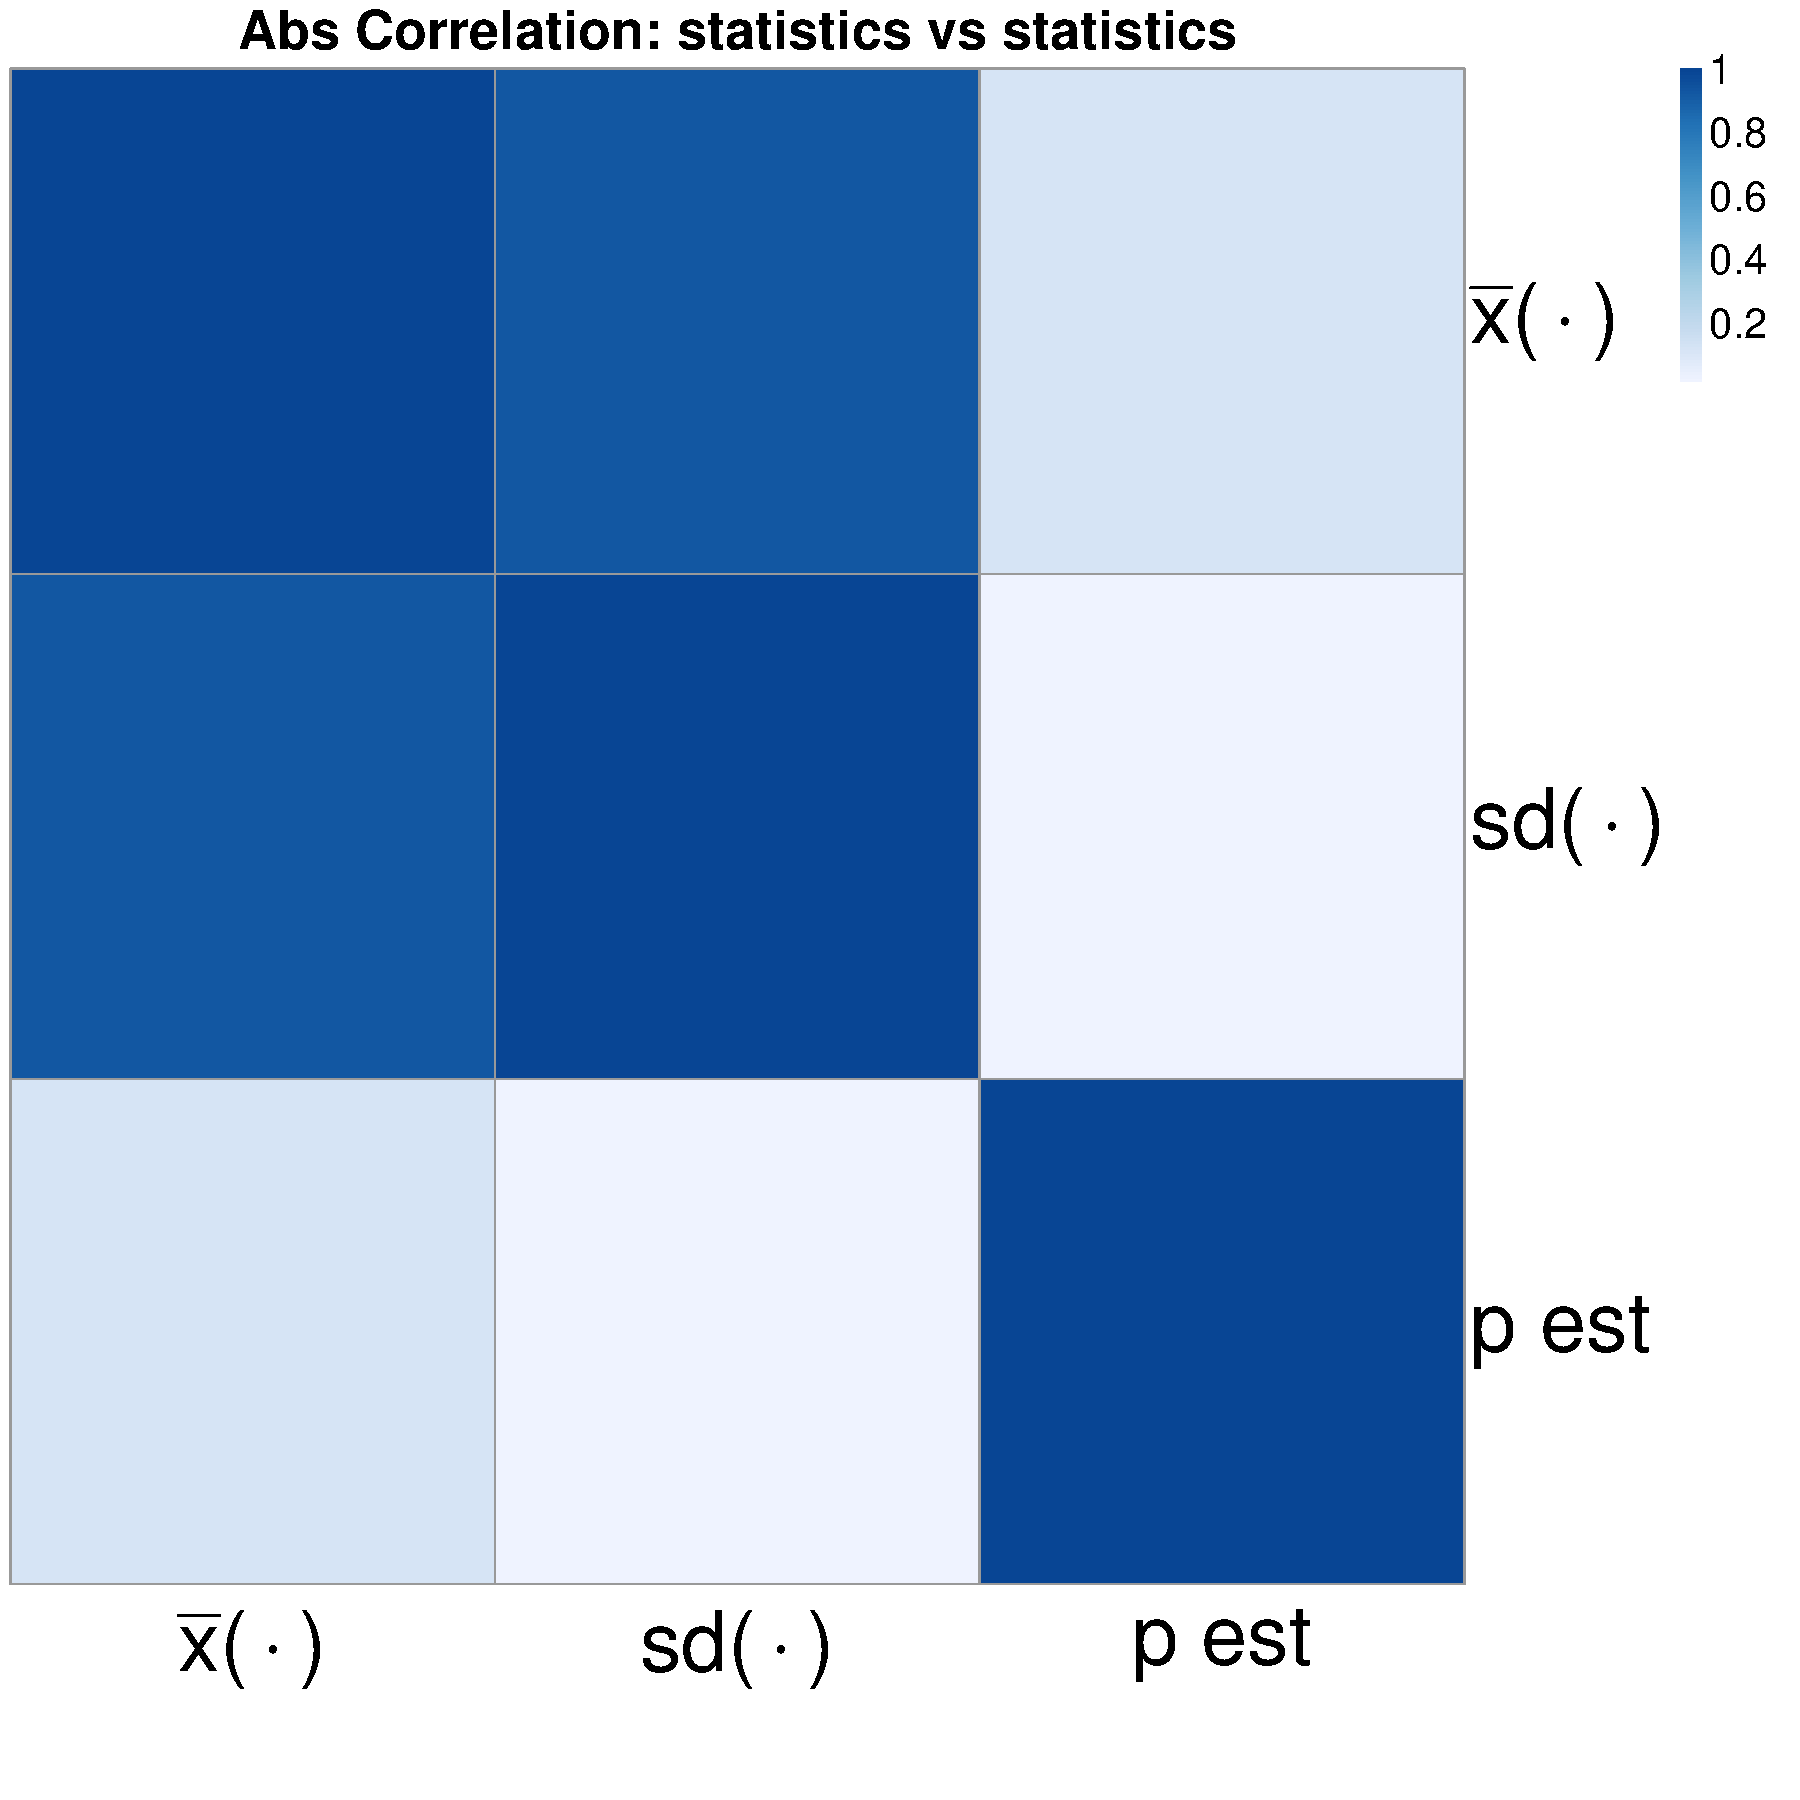
\includegraphics[width=55mm]{images/sl/gamma_example/cor_ss.pdf}}
        \caption{ZIG Example Correlation Diagrams}
        \label{fig:zigcd}
\end{figure}

The next section will take a closer look at the `ML' optimiser from \emph{Synlik} \citep{synlik_2014}.

\subsection{ML Optimiser}
The optimiser works as follows. It takes in initial values for $\pmb{\theta}$ and an initial covariance $\Sigma$. Then it samples $n$ parameters from $\mathcal{N}(\pmb{\theta}, \Sigma)$, a multivariate Normal distribution. For each sample, the likelihood function is evaluated. It then chooses the next $\pmb{\theta}$ as a linear combination of the samples, weighted by their Synthetic Likelihood. The next $\Sigma$ is chosen to be $\alpha \Sigma$ where $\alpha \in (0,1)$ is a constant; this ensures convergence. The algorithm is precisely defined in Algorithm~\ref{alg:ml}.

\begin{singlespace}
\begin{algorithm}[H]
    \caption{ML Optimiser}
    \label{alg:ml}
    \begin{algorithmic}
        \State Let $f$ be a function that computes the Synthetic Likelihood for a set of parameters
        \State Let $\pmb{\theta}_0$ be the initial parameters
        \State Let $\Sigma$ be the initial covariance
        \State Let $n$ be the number of parameters to sample
        \State Let $N$ be the number of iterations
        \newline
        \Procedure{ML}{$f,\pmb{\theta}_0, \Sigma, n, N, \alpha$}
            \State $\Theta \gets $ Empty matrix of dimensions $N + 1 \times \text{dim}(\pmb{\theta}_0)$
            \State $\Theta_{1*} \gets \pmb{\theta}_0^T$
            \For{$i$ in $1$:$N$}
                \State $P \gets n$ samples from $\mathcal{N}(\Theta_{i*}, \Sigma)$
                \State $\pmb{l} \gets (f(P_{j*}))_{j=1}^n$
                \State Discard any undefined likelihoods from $\pmb{l}$ and the corresponding rows of $P$
                \State Let $n_2$ be the number of well-defined likelihoods
                \State Define $g(x) = e^{x - m}$ where $m = \max{\{l_1, \ldots, l_{n_2}\}}$
                \State $\pmb{u} \gets (g(l_j))_{j=1}^{n_2}$
                \State $\pmb{w} \gets (\sum_{j=1}^{n_2} u_j)^{-1} \pmb{u}$
                \State Obtain $X_1$ by subtracting $\Theta_{i*}$ from each row of $P$
                \State Obtain $X_2$ by multiplying each row of $X_1$ by its corresponding weight in $\pmb{w}$
                \State Obtain $\pmb{v}$ by summing each column of $X_2$
                \State $\pmb{\theta}_1 \gets (\Theta_{ij} - v_j)_{j=1}^{\text{dim}{(\pmb{\theta}_0})}$
                \State $\Theta_{i+1, *} \gets \pmb{\theta}_1^T$
            \EndFor
            \State \Return $\Theta$
        \EndProcedure
    \end{algorithmic}
\end{algorithm}
\end{singlespace}

The next section will provide additional important $M$-Estimators.

\subsection{\texorpdfstring{$M$}{M}-Estimators}

In Section~\ref{subsec:rcm}, it was shown that Maximum Likelihood Estimators are $M$-Estimators. In preparation for fitting Model $\mathcal{A}$, it will also be shown that Ordinary Least Squares (OLS) regression estimators and the sample mean under a quadratic loss function are also $M$-Estimators.

First, that OLS regression estimators are $M$-Estimators.

\begin{proposition}
    \label{prop:ols}
    Suppose there is data $\pmb{x}_1, \pmb{x}_2, \ldots, \pmb{x}_n, \pmb{y}$. Consider the regression $\pmb{y} = X\pmb{\beta} + \pmb{\epsilon}$ where
    \begin{equation}
        X = \begin{pmatrix}
        1 & \text{---} & \pmb{x}_1^T & \text{---} \\
        1 & \text{---} & \pmb{x}_2^T & \text{---} \\
        \vdots & \vdots & \vdots & \vdots \\
        1 & \text{---} & \pmb{x}_n^T & \text{---}
        \end{pmatrix}.
    \end{equation}
    Then, the OLS estimators $\hat{\pmb{\beta}}$ are $M$-Estimators.
\end{proposition}

\begin{proof}
    As per OLS estimation, obtain $\hat{\pmb{\beta}}$ by minimising the sum of squared residuals \citep[p.~15]{hayashi_2000}. That is
    \begin{equation}
        \hat{\pmb{\beta}} = \argmin_{\pmb{\beta}} \sum_{i=1}^n \epsilon_i^2 = \argmin_{\pmb{\beta}} \sum_{i=1}^n (y_i - X_{i*} \pmb{\beta})^2.
    \end{equation}
    Thus, taking $\rho(X_{i*}, y_i, \pmb{\beta}) = (y_i - X_{i*} \pmb{\beta})^2$ satisfies what is needed for $\hat{\pmb{\beta}}$ to be an $M$-Estimator.
\end{proof}

Second, that the sample mean with the quadratic loss function is an $M$-Estimator.

\begin{proposition}
    \label{prop:squared-loss}
    Consider data $\pmb{x} \in \mathbb{R}^n$. Then the sample mean $\bar{x} = \frac{1}{n} \sum_{i=1}^n x_i$ minimises the quadratic loss $L(\xi) = \frac{1}{2} \sum_{i=1}^n (x_i - \xi)^2$ and is thus an $M$-Estimator.
\end{proposition}

\begin{proof}
    Taking the first derivative with respect to $\xi$ yields
    \begin{equation}
        \frac{\dif{L}}{\dif{\xi}}(\xi) = \sum_{i=1}^n(\xi - x_i) = n\xi - \sum_{i=1}^n x_i.
    \end{equation}
    So $L$ has a unique stationary point at $\xi = \bar{x}$. Taking the second derivative reveals
    \begin{equation}
        \frac{\dif^2{L}}{\dif{\xi^2}}(\xi) = n > 0
    \end{equation}
    so $\xi = \bar{x}$ is the unique minimum of $L$ and thus sample mean $\bar{x}$ with the quadratic loss function is an $M$-Estimator.
\end{proof}

Finally, before fitting Model $\mathcal{A}$, the asymptotic normality of $M$-Estimators will be presented.

\subsection{Asymptotic Normality of \texorpdfstring{$M$}{M}-Estimators}
\label{subsec:theoretical-properties}

For the purposes of this section, $\to_{\mathcal{D}}$ will denote convergence in distribution and $\to_{\mathbb{P}}$ will denote convergence in probability.

The goal will be to show that an $M$-Estimator is asymptotically normal in the following sense. Suppose $X_1, X_2, \dots$ are independent and identically distributed random variables. Also suppose $(\hat{\theta}_n)$ is a sequence of $M$-estimators. That is
\begin{equation}
    \label{eqn:estimators}
    \hat{\theta}_n = \argmin_{\theta} \sum_{i=1}^n \rho(X_i, \theta)
\end{equation}
for some function $\rho$. Then, under certain conditions and using `sloppy' asymptotics $\hat{\theta}_n \approx \mathcal{N}(\theta^*, \tilde{\Sigma})$ where
\begin{equation}
    \theta^* = \argmin_{\theta} \mathbb{E} \rho(X_1, \theta)
\end{equation}
and $\tilde{\Sigma}$ is the Robust Covariance Matrix. This is an important theorem as it justifies the use of the Robust Covariance Matrix and the multivariate Normal assumption for Synthetic Likelihood Estimation.

First, a sketch proof will be presented, following the approach from \cite{geyer_2013}. Then, a more rigorous theorem from \cite{pollard_1985} will be stated but not proved.

Define $\lambda(\theta) = \mathbb{E} \rho(X_1, \theta)$. Assume $\lambda$ achieves its minimum at some point $\theta^*$ on the interior of the parameter space. So $\lambda'(\theta^*) = 0$. Next, write $\rho_n(\theta) = \sum_{i=1}^n \rho(X_i, \theta)$. Now, define
\begin{equation}
    V_n(\theta) = \text{var}(\rho'_n(\theta))
\end{equation}
and
\begin{equation}
    J_n(\theta) = -\mathbb{E}\rho''_n(\theta).
\end{equation}
By properties of the variance and expectation, $V_n(\theta) = nV_1(\theta)$ where $V_1(\theta) = \text{var}(\rho'(X_1, \theta))$ and  $J_n(\theta) = nJ_1(\theta)$ where $J_1(\theta) = \mathbb{E}\rho''(X_1, \theta)$. Now, under some technical conditions and the law of large numbers
\begin{equation}
    -\frac{1}{n}\rho''_n(\theta^*) \to_\mathbb{P} J_1(\theta^*)
\end{equation}
and using the central limit theorem,
\begin{equation}
    \frac{1}{\sqrt{n}} \rho'_n(\theta^*) \to_\mathcal{D} \mathcal{N}(0, V_1(\theta^*)).
\end{equation}
Considering the Taylor expansion of $\rho'_n$ around $\theta^*$ (this is justified for large $n$ since it turns out $\hat{\theta}_n$ is consistent) reveals
\begin{equation}
    \label{eqn:taylor}
    \rho'_n(\hat{\theta}_n) \approx \rho'_n(\theta^*) + \rho''_n(\theta^*)(\hat{\theta}_n - \theta^*).
\end{equation}
Since $\hat{\theta}_n$ minimises $\rho_n(\theta)$, it must be that $\rho'(\hat{\theta}_n) = 0$. Thus, setting the right hand side of Equation~\ref{eqn:taylor} to zero yields
\begin{equation}
    \sqrt{n}(\hat{\theta}_n - \theta^*) \approx \frac{-\frac{1}{\sqrt{n}}\rho'_n(\theta^*)}{\frac{1}{n}\rho''_n(\theta^*)}.
\end{equation}
Thus, an application of Slutsky's theorem gives
\begin{equation}
    \sqrt{n}(\hat{\theta}_n - \theta^*) \to_\mathcal{D} \mathcal{N}(0, J_1(\theta^*)^{-1} V_1(\theta^*) J_1(\theta^*)^{-1}).
\end{equation}
which is \emph{almost} what was desired. To finish it off, a second use of Slutsky's theorem with the consistency of $\hat{\theta}_n$ and applying `sloppy' asymptotics yields
\begin{equation}
    \hat{\theta}_n \approx \mathcal{N}(\theta^*, \hat{J}_n(\hat{\theta}_n)^{-1} \hat{V}_n(\hat{\theta}_n) \hat{J}_n(\hat{\theta}_n)^{-1})
\end{equation}
where $\hat{J}_n(\theta) = - \rho''_n(\theta)$, the observed Fisher Information and $\hat{V}_n(\theta) = \sum_{i=1}^n \rho'_n(\theta)^2$.
This sketch proof works almost identically if $\theta$ is a vector instead of a scalar. In this case, $\hat{J}_n$ is the Hessian and $\hat{V}_n$ is the covariance of the gradient of  $\rho_n$. Thus, $\hat{J}_n(\hat{\theta}_n)^{-1} \hat{V}_n(\hat{\theta}_n) \hat{J}_n(\hat{\theta}_n)^{-1}$ is \emph{precisely} the Robust Covariance Matrix.

Now for a more rigorous theorem from \cite{pollard_1985}. First, stochastic differentibility will be defined. Then, the theorem itself will be stated.

\begin{definition}
    Let $\rho$ be a function and $\theta^*$ a point on the interior of the domain of $\rho$. Stochastic differentiability of $\rho$ at $\theta^*$ means there exists a linear approximation of $\rho$ near $\theta^*$ with remainder term $r(x,\theta)$ that is small `in an average sense' compared with $|\theta - \theta^*|$. Concretely, it is possible to write
    \begin{equation}
        \label{eqn:stoch-diff-form}
        \rho(x, \theta) = \rho(x, \theta^*) + (\theta - \theta^*)^T \Delta(x) + |\theta - \theta^*|r(x,\theta)
    \end{equation}
    where $\Delta$ denotes a vector of functions that depend only on $x$.
\end{definition}

A more rigorous definition of what it means for $r(x,\theta)$ to be small `in an average sense' compared with $|\theta - \theta^*|$ is given in \cite{pollard_1985} as the Stochastic Differentiability Condition. Now for the theorem.

\begin{theorem}
\label{the:aymp}
    Let $X_1, X_2, \ldots$ be independent observations from a distribution $P$. Write $\mathcal{P}f = \frac{1}{n} \sum_{i=1}^n f(X_i)$ for some function f. Let $(\hat{\theta}_n)$ be the sequence of estimators defined as in Equation~\ref{eqn:estimators}. Suppose
    \begin{enumerate}
        \item $G(\theta) := \mathbb{E}\rho(X_1, \theta)$ has invertible second derivative $-J$ at its maximising value $\theta^*$;
        \item $\theta^*$ is an interior point of the parameter space;
        \item $\hat{\theta}_n \to_{\mathbb{P}} \theta^*$;
        \item $\rho$ is stochastically differentiable as per Equation~\ref{eqn:stoch-diff-form};
        \item Vector $\Delta$ in Equation~\ref{eqn:stoch-diff-form} satisfies $\mathcal{P}\Delta = 0$ and $\mathcal{P}|\Delta|^2 < \infty$.
    \end{enumerate}
    Then $\sqrt{n}(\hat{\theta}_n - \theta^*) \to_{\mathcal{D}} \mathcal{N}(0, J^{-1}\mathcal{P}(\Delta \Delta^T)J^{-1})$.
\end{theorem}

The result of this theorem matches what was found with the sketch proof but is more rigorous. The conclusion is that using the Robust Covariance Matrix as the covariance of a multivariate Normal distribution and the multivariate Normal assumption are justified.

The next section will fit Model $\mathcal{A}$ using Synthetic Likelihood Estimation.